%%%%%%%%%%%%%%%
% EFT Paper
% v.2.1
% R. Itay & B. Farmer & A. Manfredini
%%%%%%%%%%%%%%%

%\RequirePackage{lineno}
\documentclass[twocolumn, %showpacs, showkeys, linenumbers 
amsmath, amssymb, amsfonts, floatfix, superscriptaddress,notitlepage]{revtex4-1} 

\usepackage[colorlinks=true, citecolor=green, filecolor=blue, linkcolor=blue, urlcolor=blue, pdfencoding=auto]{hyperref}
%\usepackage{amsfonts}
\usepackage{color}
\usepackage{placeins} % floatbarrier definition
\usepackage{graphicx}
\usepackage[perpage]{footmisc}
\usepackage[normalem]{ulem}
\newcommand \Leff{\mathcal{L}_{\mathrm{eff}}}
\newcommand \Ly{L_{\mathrm{y}}}
\newcommand \Qy{\mathcal{Q}_{\mathrm{y}}}
\newcommand \keVcc{\mathrm{keV}/\mathrm{c}^2}
\newcommand \keVr{\mathrm{keV_\mathrm{nr}}}
\newcommand \keVee{\mathrm{keV_\mathrm{ee}}}
\newcommand{\Xehund}{{XENON100}} 
\newcommand{\Xeten}{{XENON10}}
\newcommand{\Xe}{{\sc Xe}}
\newcommand{\n}[1]{\mathrm{#1}}
\newcommand{\RanComment}[1]{\textcolor{blue}{#1}}
\newcommand{\ale}[1]{\textcolor{red}{#1}}
\newcommand{\BenComment}[1]{\textcolor{green}{#1}}
\newcommand{\Ale}[1]{\textcolor{blue}{#1}}
\newcommand{\cc}[1]{$c_{#1}^2\timesm_{Weak}^4$}
\newcommand \Llike{\mathfrak{L}}
\newcommand{\Si}{\ensuremath{\mathrm{S1}}}
\newcommand{\Sii}{\ensuremath{\mathrm{S2}}}
\newcommand{\cSi}{\ensuremath{\mathrm{cS1}}}
\newcommand{\cSiib}{\ensuremath{\mathrm{cS2}_\mathrm{b}}}
\newcommand\numberthis{\addtocounter{equation}{1}\tag{\theequation}}
\allowdisplaybreaks

%%%%%%
% For rendering code example in appendix
\usepackage{listings}
\usepackage{color}
\usepackage{fancyvrb}

\definecolor{dkgreen}{rgb}{0,0.6,0}
\definecolor{gray}{rgb}{0.5,0.5,0.5}
\definecolor{mauve}{rgb}{0.58,0,0.82}

\lstset{frame=tb,
  language=Python,
  aboveskip=3mm,
  belowskip=3mm,
  showstringspaces=false,
  columns=flexible,
  basicstyle={\small\ttfamily},
  numbers=none,
  %numberstyle=\tiny\color{gray},
  keywordstyle=\color{blue},
  commentstyle=\color{dkgreen},
  stringstyle=\color{mauve},
  breaklines=true,
  breakatwhitespace=true,
  tabsize=3
}

%%%%%%%%%
\newcommand{\bern}{\affiliation{Albert Einstein Center for Fundamental Physics, University of Bern, 3012 Bern, Switzerland}}

\newcommand{\bologna}{\affiliation{Department of Physics and Astrophysics, University of Bologna and INFN-Bologna, 40126 Bologna, Italy}}

\newcommand{\chicago}{\affiliation{Department of Physics \& Kavli Institute of Cosmological Physics, University of Chicago, Chicago, IL 60637, USA}}

\newcommand{\coimbra}{\affiliation{LIBPhys, Department of Physics, University of Coimbra, 3004-516 Coimbra, Portugal}}

\newcommand{\columbia}{\affiliation{Physics Department, Columbia University, New York, NY 10027, USA}}

\newcommand{\lngs}{\affiliation{INFN-Laboratori Nazionali del Gran Sasso and Gran Sasso Science Institute, 67100 L'Aquila, Italy}}

\newcommand{\mainz}{\affiliation{Institut f\"ur Physik \& Exzellenzcluster PRISMA, Johannes Gutenberg-Universit\"at Mainz, 55099 Mainz, Germany}}

\newcommand{\heidelberg}{\affiliation{Max-Planck-Institut f\"ur Kernphysik, 69117 Heidelberg, Germany}}

\newcommand{\munster}{\affiliation{Institut f\"ur Kernphysik, Westf\"alische Wilhelms-Universit\"at M\"unster, 48149 M\"unster, Germany}}

\newcommand{\nikhef}{\affiliation{Nikhef and the University of Amsterdam, Science Park, 1098XG Amsterdam, Netherlands}}

\newcommand{\nyuad}{\affiliation{New York University Abu Dhabi, Abu Dhabi, United Arab Emirates}}

\newcommand{\purdue}{\affiliation{Department of Physics and Astronomy, Purdue University, West Lafayette, IN 47907, USA}}

\newcommand{\rpi}{\affiliation{Department of Physics, Applied Physics and Astronomy, Rensselaer Polytechnic Institute, Troy, NY 12180, USA}}

\newcommand{\rice}{\affiliation{Department of Physics and Astronomy, Rice University, Houston, TX 77005, USA}}

\newcommand{\stockholm}{\affiliation{Oskar Klein Centre, Department of Physics, Stockholm University, AlbaNova, Stockholm SE-10691, Sweden}}

\newcommand{\subatech}{\affiliation{SUBATECH, IMT Atlantique, CNRS/IN2P3, Universit\'e de Nantes, Nantes 44307, France}}

\newcommand{\torino}{\affiliation{INFN-Torino and Osservatorio Astrofisico di Torino, 10125 Torino, Italy}}

\newcommand{\ucla}{\affiliation{Physics \& Astronomy Department, University of California, Los Angeles, CA 90095, USA}}

\newcommand{\ucsd}{\affiliation{Department of Physics, University of California, San Diego, CA 92093, USA}}

\newcommand{\wis}{\affiliation{Department of Particle Physics and Astrophysics, Weizmann Institute of Science, Rehovot 7610001, Israel}}

\newcommand{\zurich}{\affiliation{Physik-Institut, University of Zurich, 8057  Zurich, Switzerland}}

\newcommand{\paris}{\affiliation{LPNHE, Université Pierre et Marie Curie, Université Paris Diderot, CNRS/IN2P3, Paris 75252, France}}

\newcommand{\freiburg}{\affiliation{Physikalisches Institut, Universit\"at Freiburg, 79104 Freiburg, Germany}}


\begin{document}

\title{Effective field theory search for high-Energy nuclear recoils using the \Xehund\ dark matter detector}

\author{E.~Aprile}\columbia

\author{J.~Aalbers}\nikhef

\author{F.~Agostini}\lngs\bologna

\author{M.~Alfonsi}\mainz

\author{F.~D.~Amaro}\coimbra

\author{M.~Anthony}\columbia

\author{F.~Arneodo}\nyuad

\author{P.~Barrow}\zurich

\author{L.~Baudis}\zurich

\author{B.~Bauermeister}\stockholm

\author{M.~L.~Benabderrahmane}\nyuad
\author{T.~Berger}\rpi

\author{P.~A.~Breur}\nikhef

\author{A.~Brown}\nikhef

\author{E.~Brown}\rpi

\author{S.~Bruenner}\heidelberg

\author{G.~Bruno}\lngs

\author{R.~Budnik}\wis

\author{L.~B\"utikofer}\altaffiliation[]{Also at Albert Einstein Center for Fundamental Physics, University of Bern, Bern, Switzerland}\freiburg

\author{J.~Calv\'en}\stockholm

\author{J.~M.~R.~Cardoso}\coimbra

\author{M.~Cervantes}\purdue

\author{D.~Cichon}\heidelberg

\author{D.~Coderre}\altaffiliation[]{Also at Albert Einstein Center for Fundamental Physics, University of Bern, Bern, Switzerland}\freiburg

\author{A.~P.~Colijn}\nikhef

\author{J.~Conrad}\altaffiliation{Wallenberg Academy Fellow}\stockholm

\author{J.~P.~Cussonneau}\subatech

\author{M.~P.~Decowski}\nikhef

\author{P.~de~Perio}\columbia

\author{P.~Di~Gangi}\bologna

\author{A.~Di~Giovanni}\nyuad

\author{S.~Diglio}\subatech

\author{G.~Eurin}\heidelberg

\author{J.~Fei}\ucsd

\author{A.~D.~Ferella}\stockholm

\author{A.~Fieguth}\munster

\author{W.~Fulgione}\lngs\torino

\author{A.~Gallo Rosso}\lngs

\author{M.~Galloway}\zurich

\author{F.~Gao}\columbia

\author{M.~Garbini}\bologna

\author{C.~Geis}\mainz

\author{L.~W.~Goetzke}\columbia

\author{Z.~Greene}\columbia

\author{C.~Grignon}\mainz

\author{C.~Hasterok}\heidelberg

\author{E.~Hogenbirk}\nikhef

\author{R.~Itay}\email[E-mail: ]{ran.itay@weizmann.ac.il}\wis

\author{B.~Kaminsky}\altaffiliation[]{Also at Albert Einstein Center for Fundamental Physics, University of Bern, Bern, Switzerland}\freiburg

\author{S.~Kazama}\zurich

\author{G.~Kessler}\zurich

\author{A.~Kish}\zurich

\author{H.~Landsman}\wis

\author{R.~F.~Lang}\purdue

\author{D.~Lellouch}\wis

\author{L.~Levinson}\wis

\author{Q.~Lin}\columbia

\author{S.~Lindemann}\heidelberg\freiburg

\author{M.~Lindner}\heidelberg%\date{\today}


\author{F.~Lombardi}\ucsd

\author{J.~A.~M.~Lopes}\altaffiliation[Also with ]{Coimbra Engineering Institute, Coimbra, Portugal}\coimbra

\author{A.~Manfredini}\email[E-mail: ]{alessandro.manfredini@weizmann.ac.il}\wis 

\author{I.~Maris}\nyuad

\author{T.~Marrod\'an~Undagoitia}\heidelberg

\author{J.~Masbou}\subatech

\author{F.~V.~Massoli}\bologna

\author{D.~Masson}\purdue

\author{D.~Mayani}\zurich

\author{M.~Messina}\columbia

\author{K.~Micheneau}\subatech

\author{A.~Molinario}\lngs

\author{K.~Mor\aa}\stockholm

\author{M.~Murra}\munster

\author{J.~Naganoma}\rice

\author{K.~Ni}\ucsd

\author{U.~Oberlack}\mainz

\author{P.~Pakarha}\zurich

\author{B.~Pelssers}\stockholm

\author{R.~Persiani}\subatech

\author{F.~Piastra}\zurich

\author{J.~Pienaar}\purdue

\author{V.~Pizzella}\heidelberg

\author{M.-C.~Piro}\rpi

\author{G.~Plante}\columbia

\author{N.~Priel}\wis

\author{L.~Rauch}\heidelberg

\author{S.~Reichard}\purdue

\author{C.~Reuter}\purdue

\author{A.~Rizzo}\columbia

\author{S.~Rosendahl}\munster

\author{N.~Rupp}\heidelberg

\author{J.~M.~F.~dos~Santos}\coimbra

\author{G.~Sartorelli}\bologna

\author{M.~Scheibelhut}\mainz

\author{S.~Schindler}\mainz

\author{J.~Schreiner}\heidelberg

\author{M.~Schumann}\freiburg

\author{L.~Scotto~Lavina}\paris

\author{M.~Selvi}\bologna

\author{P.~Shagin}\rice

\author{M.~Silva}\coimbra

\author{H.~Simgen}\heidelberg

\author{M.~v.~Sivers}\altaffiliation[]{Also at Albert Einstein Center for Fundamental Physics, University of Bern, Bern, Switzerland}\freiburg

\author{A.~Stein}\ucla

\author{D.~Thers}\subatech

\author{A.~Tiseni}\nikhef

\author{G.~Trinchero}\torino

\author{C.~Tunnell}\nikhef\chicago

\author{M.~Vargas}\munster

\author{H.~Wang}\ucla

\author{Z.~Wang}\lngs

\author{Y.~Wei}\zurich

\author{C.~Weinheimer}\munster

\author{J.~Wulf}\zurich

\author{J.~Ye}\ucsd

\author{Y.~Zhang.}\columbia

\collaboration{XENON Collaboration}\email[E-mail: ]{xenon@lngs.infn.it}\noaffiliation

\author{B.~Farmer}\email[E-mail: ]{benjamin.farmer@fysik.su.se}\stockholm

\date{\today}

\begin{abstract} 

We report on WIMP search results in the \Xehund\ detector using a non-relativistic effective field theory approach. The data from science run II (34 kg $\times$ 224.6 live days) was re-analyzed, with an increased recoil energy interval compared to previous analyses, ranging from $(6.6 - 240)~\keVr$. The data is found to be compatible with the background-only hypothesis. We present 90\% confidence level exclusion limits on the coupling constants of WIMP-nucleon effective operators using a binned profile likelihood method. We also consider the case of inelastic WIMP scattering, where incident WIMPs may up-scatter to a higher mass state, and set exclusion limits on this model as well. 
\end{abstract}

\pacs{}
\keywords{Dark Matter, EFT, Xenon}

\maketitle 


\section{Introduction}
%	Astrophysical and cosmological observations present evidence that 27\% of the mass-energy of the Universe is made out of Dark Matter (DM), a non-luminous, non-baryonic and non-relativistic particle, though the nature of this particle is yet unknown~\cite{Harvey1462}. While several types of new DM candidate raise from many theories, the most prominent one is the Weakly Interacting Massive Particles(WIMPs)~\cite{Bertone:2010zza}. Many  direct detection experiments attempt to measure the rare scattering of WIMPs from target nucleus. Although some experiment see an excess for WIMPs in the mass range of 6-30 GeV/$C^2$~\cite{DAMA,COGENT,CDMSlite,CREST}, these results are in tension with other experiments~\cite{xe100_run_combination,PANDAX,LUXnew}.

Astrophysical and cosmological observations provide strong evidence that 27\% of the \RanComment{energy density} of the universe is made out of Dark Matter (DM), a non-luminous, non-baryonic, and non-relativistic particle, the nature of which is yet unknown~\cite{Harvey1462,WMAP:9years,PLANCK}. Many well-motivated theoretical extensions of the Standard Model of particle physics predict the existence of one or more particles with the required properties, with masses \RanComment{and cross sections} typically of the order of the weak scale. Such particles are collectively known as Weakly Interacting Massive Particles(WIMPs)~\cite{Bertone:2010zza}. The hypothesis that dark matter is constituted primarily of WIMPs is currently being tested by many experiments, either indirectly by seaching for evidence of their possible decay or annihilation in astrophysical processes, by searching for evidence of their direct production at collider experiments, or by directly measuring the rare scattering of astrophysical WIMPs from target nuclei in Earth-based laboratories. We report on a search of this last kind. Although \RanComment{there are} still reported potential evidence for WIMPs in the mass range of 6-30 GeV/$c^2$~\cite{DAMA,}, these results appear to conflict with null results from other experiments~\cite{xe100_run_combination,PANDAX,LUXnew,COGENT,CDMSlite,CREST}.

%	 Typically the standard calculation for WIMP-nucleon scattering simplifies the type of interaction to Spin Independent (SI) and Spin Dependent (SD) interactions~\cite{LEWIN}, however these are not the only possible types of interactions. In recent years an Effective Field Theory (EFT) approach that takes into account all leading-order and next-to-leading order operators that emerge from an effective Lagrangian describing the WIMP-nucleus interaction has been developed ~\cite{Fitzpatrick:2012ib,Anand:MathTools,Fitzpatrick:MathTools}. In this framework new operators which come from different type of nuclear responses are introduced along with the standard SI and SD ones. The parametrization of the fourteen operators $\mathcal{O}_i$ is listed in Eq.~\ref{eq:OpDef} and follows the convention from~\cite{Anand:MathTools}. The operators dependence explicitly on 4 quantities: $\vec{v}^{\perp}$, the relative velocity between the WIMP and the nucleon, $\vec{q}$, the momentum transfer, and the WIMP and nucleon spin $\vec{S}_\chi$ , $\vec{S}_N$. Notice that $\mathcal{O}_2$ is not treated as it cannot be obtained from a relativistic operator at leading order.

The traditional approach for computing predictions of the rate of WIMP-nucleon scattering has been to take only leading-order terms in a WIMP-nucleon effective field theory (EFT) with a very simple treatment of nuclear structure~\cite{LEWIN}. This leads to two main types of interactions, which are commonly labelled ``Spin Independent'' (SI) and ``Spin Dependent'' (SD), however in recent years many authors have been pointed out that in certain theories these interactions may be suppressed or nonexistent, such that otherwise subleading interactions may dominate the scattering process. To account for this possibility in a systematic way a more sophisticated EFT approach has been developed ~\cite{Fitzpatrick:2012ib,Anand:MathTools,Fitzpatrick:MathTools}, which takes into account all leading-order and next-to-leading order operators emerging from an effective Lagrangian describing the WIMP-nucleus interaction. In this framework new operators associated with different types of nuclear responses are introduced along with the standard SI and SD ones, resulting in a set of fourteen operators $\mathcal{O}_i$ which may each couple independently to protons and neutrons. In Eq.~\ref{eq:OpDef} we list these operators following the convention from~\cite{Anand:MathTools}. The operators depend explicitly on 4 linearly independent quantities: $\vec{v}^{\perp} \equiv \vec{v} + \frac{\vec{q}}{2\mu_N} $, the relative perpendicular velocity between the WIMP and the nucleon, $\vec{q}$, the momentum transferred in the scattering event, and $\vec{S}_\chi$, $\vec{S}_N$, the WIMP and nucleon spins. $\mathcal{O}_2$ is not considered here as it cannot be obtained from a relativistic operator at leading order.

\begin{align*} 
&\mathcal{O}_1 = 1_{\chi} 1_N  \\
%&\mathcal{O}_2 = (v^{\perp})^2 \\
&\mathcal{O}_3 = i\vec{S}_N\cdot (\frac{\vec{q}}{m_N}\times\vec{v}^\perp) \\
&\mathcal{O}_4 = \vec{S}_{\chi}\cdot \vec{S}_N \\
&\mathcal{O}_5 = i\vec{S}_{\chi}\cdot (\frac{\vec{q}}{m_N}\times\vec{v}^\perp) \\
&\mathcal{O}_6 = (\vec{S}_{\chi} \cdot \frac{\vec{q}}{m_N})(\vec{S}_N \cdot \frac{\vec{q}}{m_N}) \\
&\mathcal{O}_7 = \vec{S}_N \cdot \vec{v}^\perp \\
&\mathcal{O}_8 = \vec{S}_{\chi} \cdot \vec{v}^\perp \numberthis \label{eq:OpDef} \\
&\mathcal{O}_9 = i\vec{S}_{\chi} \cdot(\vec{S}_N \times \frac{\vec{q}}{m_N}) \\
&\mathcal{O}_{10} = i\vec{S}_N \cdot (\frac{\vec{q}}{m_N}) \\
&\mathcal{O}_{11} = i\vec{S}_{\chi} \cdot (\frac{\vec{q}}{m_N}) \\
&\mathcal{O}_{12} = \vec{S}_\chi \cdot (\vec{S}_N \times \vec{v}^\perp) \\
&\mathcal{O}_{13} = i(\vec{S}\chi \cdot \vec{v}^\perp)(\vec{S}_N \cdot \frac{\vec{q}}{m_N})\\
&\mathcal{O}_{14} = i(\vec{S}_\chi \cdot \frac{\vec{q}}{m_N})(\vec{S}_N \cdot \vec{v}^\perp) \\
&\mathcal{O}_{15} = -(\vec{S}_\chi \cdot \frac{\vec{q}}{m_N})[(\vec{S}_N \times \vec{v}^\perp)\cdot \frac{\vec{q}}{m_N}]
\end{align*}

 
%	    Unlike The formally studied types of interaction (SI,SD) which are not suppressed when $\vec{q} \rightarrow 0$ and most of their interaction rate will be in low energies recoils, some of the new operators depend explicitly on $\vec{q}$ therefore their interaction rate is suppressed with $\vec{q}$ and peaks at higher energies than previously looked in direct detection experiments ($< 43$ keV), and hence could not be treated before see Fig. ~\ref{fig:dRdE}.
	    Unlike the more commonly studied types of interaction (SI,SD), which are not suppressed when $\vec{q} \rightarrow 0$ and for which the scattering rate on nucleons is expected to be largest for low energy nuclear recoils, some of the new EFT operators depend explicitly on $\vec{q}$ and so their interaction cross section is suppressed for low momentum transfers. Consequently, their scattering rate peaks at non-zero nuclear recoil energy, which for sufficiently high WIMP masses may even occur outside typical analysis windows ($< 43$~keV) which are designed to search for SI and SD interactions (see Figure~\ref{fig:dRdE}). Due to \RanComment{the theoretical bias high only considering SI and SD interactions, high energy nuclear recoils have remain unexplored in many experiments}.
	    
%	    Another assumption that can be relaxed is that WIMP should scatter elastically, however there are models in which the incoming and outgoing WIMPs have different mass states ~\cite{InelasticIntro}. In the case where the outgoing state is more massive than the incoming state the event rate at low recoil energies can again be suppressed, hence analyses which apply an upper energy bound lose sensitivity to these types of interactions. Recently an inelastic adaptation of the EFT operator framework discussed above was developed~\cite{InelasticMath}. The operators presented in~\ref{eq:OpDef} are modified such that $\vec{v}^\perp_{inelastic} = \vec{v}^\perp_{elastic} +\frac{\delta}{\vert{\vec{q}}\vert^2}\vec{q}$. \RanComment{We should add here the dependency of $v_{min}$ on $\delta$}      
	    Another typical assumption that can be relaxed is that WIMPs should scatter elastically with nuclei, however there exist dark matter models in which the incoming and outgoing WIMPs have different mass states ~\cite{InelasticIntro} separated by a keV-scale splitting. In the case where the outgoing state is more massive than the incoming state the cross section for low recoil energies can again be suppressed, this time by the scattering kinematics. Recently an inelastic adaptation of the EFT operator framework discussed above was developed~\cite{InelasticMath}. In this case the operators presented in Eq.~\ref{eq:OpDef} are modified such that $\vec{v}^\perp_{inelastic} = \vec{v}^\perp_{elastic} +\frac{\delta_m}{\vert{\vec{q}}\vert^2}\vec{q}$. We discuss this case further in section \ref{subsubsec:Inelastic}.
	    
The EFT framework of \cite{Fitzpatrick:2012ib} is constructed at the WIMP-nucleon level and so each operator may be present independently for protons and neutrons, though UV models can of course correlate their couplings. The full EFT thus has 28 coupling parameters in addition to the WIMP mass, and, in the inelastic case, a mass splitting $\delta$. The parameter space is thus too large to explore in full, so we take a similar approach to the SI/SD case and characterize the experimental limit by assuming only one active operator at a time, with the coupling to protons and neutrons for that operator set equal (the ``isoscalar'' case). However, to facilitate the full exploitation of these results by the community, we provide in supplementary material a set of tools for converting any theoretical recoil spectrum $\mathrm{d}R/\mathrm{d}E$ into an accurate event rate prediction for this analysis, including all detector response and analysis efficiency effects. This may help to set a mildly conservative but quite accurate limit on arbitrary models in the full EFT parameter space, or indeed any other particle dark matter model for which one can supply the expected recoil spectrum.

In this paper, motivated by these EFT extensions of the standard WIMP framework, we report on an analysis extending the searched recoil energy range up to 240\,keV for the first time in the \Xehund\ experiment, and present exclusion limits on all operators for both the elastic and the inelastic WIMP cases.     
%  \begin{itemize}
%  \item Motivation: dark matter, theoretical possibility of high energy recoil events. Mention some specific models, maybe inelastic scattering also.
%  \item Theoretical background on EFT operators, inc. motivation (e.g. possibility to reconcile limits vs possible signals in other experiments, model-independent approach to constraining exotic models)
%  \item (if we do it) Theoretical background on inelastic scattering kinematics.
%  \item Motivating example plots of recoil spectra/signal models (e.g. Fig. \ref{fig:dRdE}). Also discuss the lower electronic recoil background at these higher recoil energies, which improves the analysis sensitivity beyond what would be expected from the raw increase in predicted event rate (At least I presume so, need to estimate this perhaps. I think we can say something like this; the standard analysis signal region has a signal acceptance of maybe 50\% since it cuts the nuclear recoil band about in half, whereas for us it is almost 90\% since there is good separation between ER and NR bands. So for say O3 (either mass) we expect about twice as many events due to the extended signal region, with twice the acceptance in the new high PE region. So overall I guess it is roughly a factor of 3 improvement in total signal rate, and similar for the sensitivity. In fact from the proper sensitivity estimates the improvement is a little better than that, but this gives a rough idea where the improvement comes from.).
% \end{itemize}


\begin{figure}[t!]
\centerline{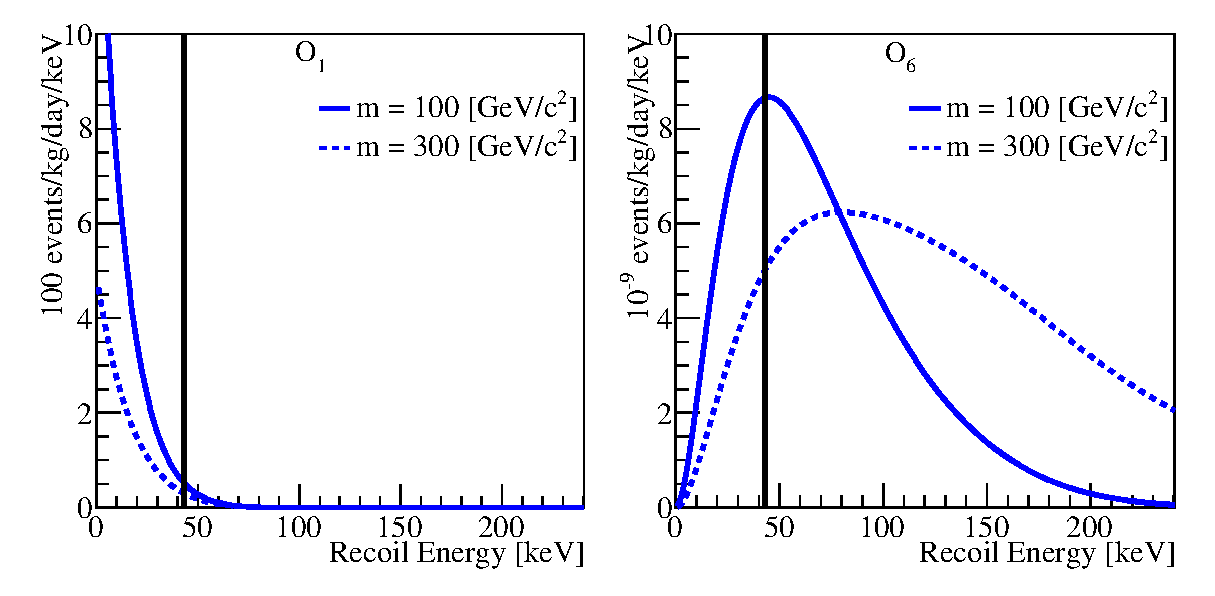
\includegraphics[width=1.\linewidth]{Figures/drdeO1O6.eps}}
\caption{Example EFT recoil spectra for elastic scattering of spin-$1/2$ WIMPs on Xenon nuclei (weighted according to the isotope abundances in the XENON100 experiment). Left(right) shows the predicted spectra for EFT operator $\mathcal{O}_1$($\mathcal{O}_6$). The normalization is controlled by the coupling coefficient of each EFT operator and the experimental exposure (left arbitrary in this figure). The solid vertical line at 43 keV shows the approximate division between the two signal regions used in this analysis (30 PE in cS1). As shown, the standard SI ($\mathcal{O}_1$) spectrum is concentrated mainly in the already explored energy region. However, some EFT operators, for certain WIMP masses, predict a significant fraction of recoil events above the upper energy cut used in the standard spin-independent analysis, motivating an extension of this cut. The highest recoil energy shown in the plots, 240\,keV, roughly corresponds to the extended $cS1$ cut of 180\,PE used in this analysis.}
\label{fig:dRdE}
\end{figure}

\section{The \Xehund\  Detector}
The \Xehund\ detector is a cylindrical %30\,cm~height, 30\,cm~diameter, 
dual-phase xenon (liquid and gas) time projection chamber (TPC). It is installed at the Laboratori Nazionali del Gran Sasso (LNGS) in Italy
and hosts 161\,kg of liquid xenon (LXe), of which 62\,kg function as the active target ~\cite{xe100_instr2012}. 
The detector consists of a total of 178~1-inch square Hamamatsu R8520-AL photomultiplier tubes (PMTs) employed in two arrays, one in the gas phase at the top of the TPC, and the other at the bottom, immersed in the LXe. 

A particle interacting with the LXe deposits energy that creates both excited and ionized molecular states. De-excitation of these excited molecular states induce a prompt scintillation signal ($S1$), while 
electrons from ionization processes are drifted in an electric field of $530$V/cm towards the liquid-gas interface where they are extracted using a larger electric field of $\sim12$kV/cm. 
These electrons generate a proportional scintillation, which is called $S2$. The spatial distribution of the $S2$ signal on the top PMT array, together with the time difference between $S1$ and $S2$ signals, provides respectively X-Y and Z position information for each interaction, allowing 3D position reconstruction to be achieved.
%determines the X-Y position, while the time difference between the two signals gives the z-coordinate, and thus a 3D position reconstructions is achieved.

Interactions in different positions cover different solid angles with respect to the PMT array, which leads to a position-dependent S1 signal. At the same time, warping of the top meshes and the absorption of electrons by residual impurities lead to a position-dependent S2 signal. To take these effects into account a correction is applied based on a light collection efficiency (LCE) map. The corrected signals (cS1,cS2) are spatially independent and uniform to all interactions~\cite{xe100_instr2012}.

The $S2/S1$ ratio is known to differ between nuclear recoil (NR) and electronic recoil (ER) interactions, and is thus used as a discriminating variable between a WIMP signal and ER background.
The logarithm of this ratio, $log(cS2/cS1)$ is referred later in the text as the $y$ discriminating variable.
% between ER background coming from $\gamma$, $\beta$ and NR signal coming from a WIMP. 



\section{Data Analysis}
\label{sec:Analysis}
%In this work we analyse the data from \Xehund's scientfic run II~\cite{xe100_run10_si,xe100_run10_sd} recorded between February 2011 and March 2012, 
In this work we perform a re-analyse of the scientfic run~II data recorded between February 2011 and March 2012, 
corresponding to 224.6~live~days. \textcolor{red}{Some words about calibration data used}. \RanComment{What do you mean , the amount of total CoTh and AmBe ? I haven't seen any explanations on this except for what are the calibration sources }

This analysis extends the previous results~\cite{xe100_run10_si,xe100_run_combination}, addressed in the following as the low energy channel , with a new study exploring the energy range between 30-180\,PE (43-240\,keV \RanComment{Make sure this value is correct!!!}) in $S1$  \textcolor{red}{maybe better to say in KeV??}. 
%However we enlarge the energy range to be 3PE-180PE. In order to preform a blind analysis we divide our work into two energy ranges. Low energy , 3PE-30PE which is identical to the range in the works mentioned above, and a high energy range, 30PE-180PE. The main emphasis of this paper is the second region, on which no work has been done yet. 
\RanComment{Thre is a bit of repetition in these two paragraphs consider revising }The data analysis is divided into two mutually exclusive channels, one optimized for low energies and ranging from 3-30\,PE in $cS1$ \RanComment{(LowE)}, the other optimized for high energies recoils
ranging from 30-180\,PE in $cS1$ \RanComment{(highE)}, which are finally statistically combined. 
The relative region of interests (ROI) of these two channels are shown in Figure~\ref{fig:phasespace} and further described in the following sections. 

\RanComment{Not sure this paper is so long we actually needs this full description, In any case I believe it is important to state the main new thing of this analysis which is the high energy part}
This section describes the analysis procedures such as selection criterion, background expectation models and signal acceptance estimation  employed
for the low and high energy channels, reported in Section~\ref{subsec:LowE} and~\ref{subsubsec:HighE} respectively. 
%This work focuses on the high energy channel, a brief description of the low evenrgy channel is reported in Section~\ref{subsec:LowE}.
\RanComment{I think maybe we should explain the S2 bottom used (might go in signal model or here)}

\subsection{Low Energy Channel}
\label{subsec:LowE}
This analysis channel relies on the re-analysis of run~II data described in~\cite{xe100_run_combination}. The region of interest (ROI), the background 
expectation models, data selections and their acceptances are mostly unchanged and so are only briefly summarized here. Differences with respect to said results are highlighted when present.

The ROI for this channel is defined in the ($y,cS1$)-plane and is shown in Figure~\ref{fig:phasespace}.  The lower 
bound on $y$ corresponds to a 3\,$\sigma$ acceptance quantile (as a function of cS1) of a 20~GeV WIMP mass signal model assuming an $\mathcal{O}_1$ (SI) interaction, while the upper bound is fixed at y\,=\,2.7.
The range in cS1 is selected as 3 to 30\,PE. 
The ROI is further divided into eight sub-regions (also called bands) depending on the operator $\mathcal{O}_i$ and on the WIMP mass hypothesis. 
These bands are arranged to achieve constant expected signal density in each region, as described in~\cite{xe100_run_combination}.

\begin{figure}[]
\begin{minipage}{1\linewidth}
\centerline{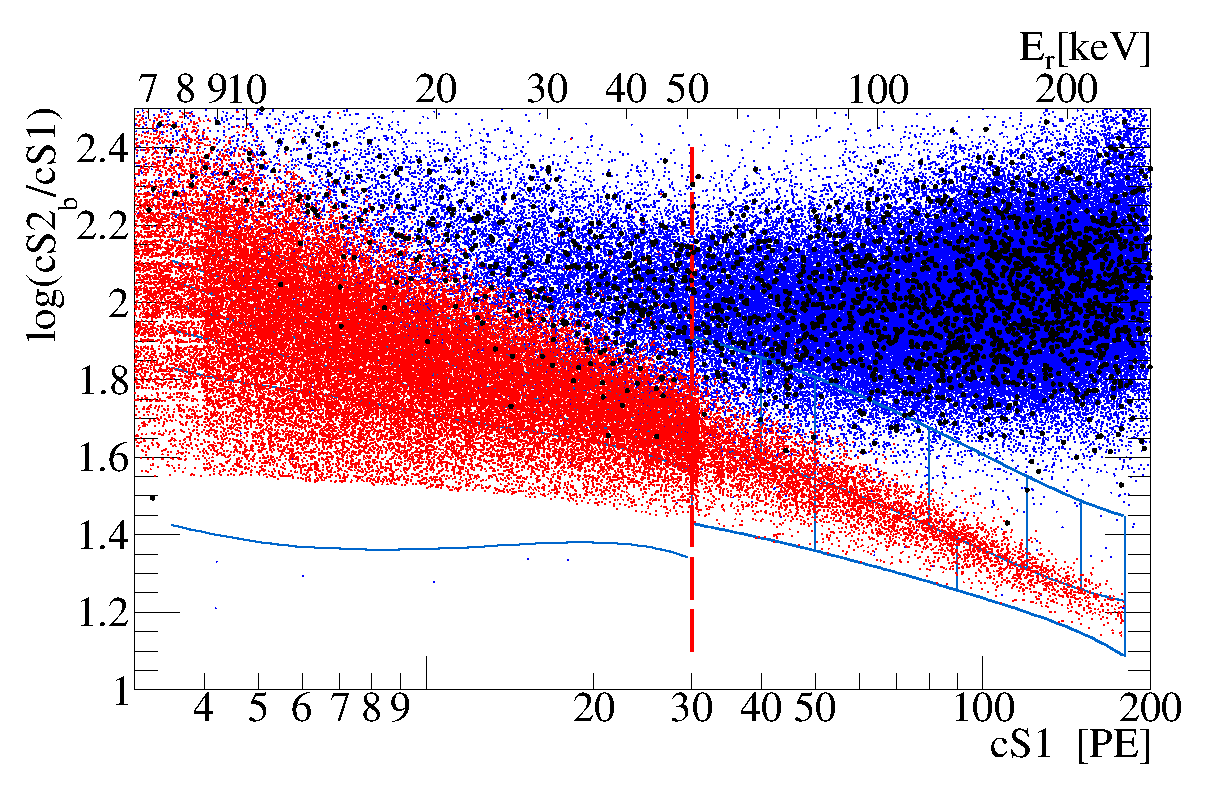
\includegraphics[width=1\linewidth]{Figures/eft_sr.eps}}
\end{minipage}
\caption{Summary of regions of interest, backgrounds, and observed data. ER calibration data, namely $^{60}\mathrm{Co}$ and $^{232}\mathrm{Th}$ data is shown as blue dots. NR calibration data ($^{241}$AmBe) is shown as red dots. Dark matter search data is shown as black dots. The red dashed line is the threshold between the low and high energy channels. The lines in blue are the bands. For the low-energy channel these are operator and mass dependent, but are shown here for a 50~GeV/$c^2$ WIMP using the $\mathcal{O}_1$ operator. For the high-energy region, the nine analysis bins are presented also in blue lines.
%\sout{the top left bin in this region is bin 1, the top right is bin 6, the bottom left is bin 7 and bottom right is bin 9. 
%In Sec.~\ref{sec:Results} we show similar data but for regions above the upper range of this analysis, going up to 1000\,PE in cS1, for completeness as part of final unblinding of XENON100 data.} 
}
\label{fig:phasespace}
\end{figure}  


Other than falling into the ROI, an event should fulfill several additional selection criteria (cuts). Data quality and selection cuts are defined to remove events with poor data quality or noisy signals. \ale{Events are discarded if they present} a time-coincident signal in the outer LXe veto, S2 signals below threshold, multiple-scatters, or are localized outside a predefined fiducial volume of 34 kg. In addition, this analysis channel uses the post-unblinding cuts and data reprocessing described in~\cite{xe100_run_combination}. More details on these selection criteria and their relative WIMP signals acceptances can be found in~\cite{Aprile:2012vw,xe100_run_combination}. 
%%%%% MAYBE THIS CAN BE COMMENTED OUT %%%%%%
%%% Ale : already sayd above, and is not "new features" of this analysis.
%\sout{To summarize the main new features in this analysis, data is reprocessed with an improved (S1,S2) classification algorithm, and a new cut targeted to suppress data periods with non-random occurrence of lone-S1 (an S1 without 
%any correlated S2) events is applied.} 
%%%%%%%%%%%%%%%%%%%%%%%%%%%%%%%%%%%%%%%%%%%%%
\ale{Note that}
%Finally, 
this analysis channel does not employ a variable lower S1 threshold as a function of the event position in the TPC, but instead applies a fixed lower threshold cut on cS1 at 3\,PE, \ale{conversely} to the choice made in~\cite{xe100_run_combination}.

The expected background is modeled separately for ER and NR contributions which are then scaled to exposure and added together.
The NR background is estimated by Monte Carlo simulation and accounts for the radiogenic and cosmogenic neutron
contributions~\cite{Aprile:2013tov}. The ER background is parametrized as the linear combination of Gaussian-shaped and non-Gaussian components.
The first is obtained via a parametric fit of the $^{60}$Co and $^{232}$Th calibration data, as discussed in~\cite{xe100_run10_si}.
%In contrast, the expected distribution and yields for the non-Gaussian population, 
\ale{The second, } consisting of anomalous events such as those 
presenting incomplete charge collection or accidental coincidence of uncorrelated S1s and S2s,  
is evaluated via dedicated techniques described in~\cite{xe100_run_combination}.

\ale{Systematic uncertainties on the background model arising from the Gaussian parametrized fit, from the normalizations of the NR and from the non-Gaussian components, have been evaluated and propagated to each band}. \BenComment{*This sentence doesn't make sense; missing an "and" or something? I can't quite guess what it is supposed to mean*} These errors are small with respect to the statistical uncertainties of each band, which are conservatively taken as the overall uncertainty~\cite{xe100_run_combination}, as discussed in Sec.~\ref{sec:LikelihoodFunction}.



\subsection{High Energy}
\label{subsubsec:HighE}

%\subsection{Analysis and Data Selection}
%\subsection{Data Selections}
%\label{subsec:AnalysisAndDataSelection}

The data selection cuts which are defined to low energy recoil only, are extended, modified or removed to be compatible with high energy recoils. Most of the cuts were fully compatible or naively extended to high energy depositions, however one cut is dropped and two are modified. In order to throw away peculiar events we compare the width of the S2 to its z-position. In this analysis we adopt a newer version of this cut, developed for scientific run III see ~\cite{xe100_run_combination}. As a WIMP will interact only once in the detector we remove events whcih have more then one S2. we adopt here a cut that is more suitable to higher energies and demands a single S2 in a 160 $\mu$S window. In order to define the interaction exact location, we use several algorithms, one of the is the Neural Network (NN), as we do not train the detector using high ER events, the NN gives a large $\chi^2$ for these events. In order to not under estimate the background we drop this cut. We do keep other cuts on position reconstruction to make sure we can fiducialize correctly for more details on all cuts see ~\cite{xe100_ana2012}. Finally the total acceptance is fitted using a 3rd order polynomial presented in Figure~\ref{fig:Acc}

\begin{figure}[h!]
\begin{minipage}{1.\linewidth}
\centerline{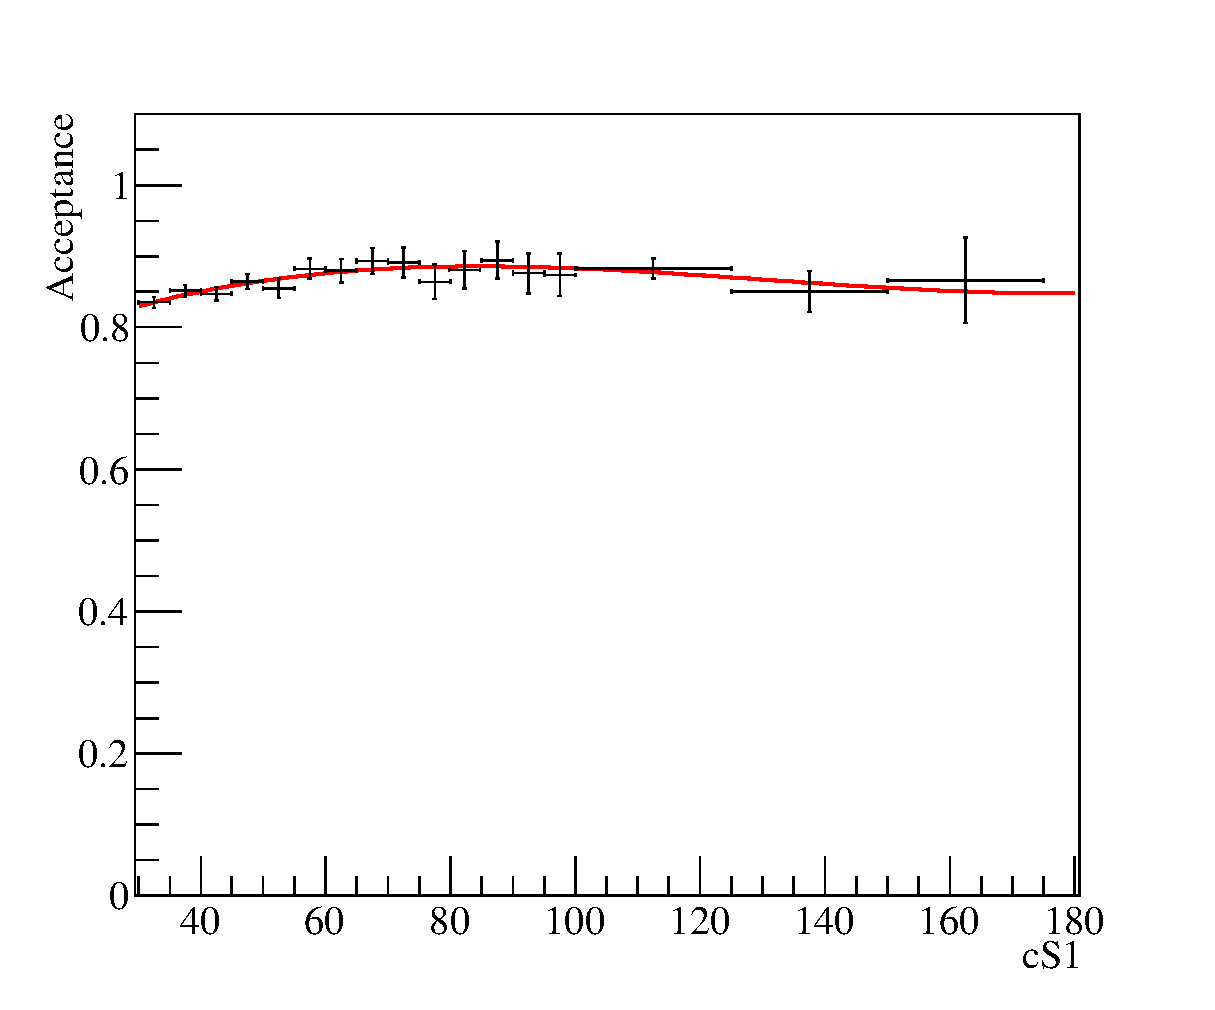
\includegraphics[width=1.\linewidth]{Figures/Acceptance.eps}}
\end{minipage}
\caption{The total acceptance of all cuts used, data from calibration in black and the fit in red.}
\label{fig:Acc}
\end{figure}

%%%%%%%%%%%%%%%%%%%%%%%%%%%%  THIS MAYBE BETTER UP, or part of it %%%%%%%%%%%%%%%%%%%%%%%%%%%%%%%%%%%%%
We define our signal region in the discrimination space (log(S2/S1) Vs S1). The upper bound is defined by taking the NR calibration sample mean and scaling it up such that in 30PE it coincide with the ER mean. From below the signal is bounded by taking 3 sigma from the NR mean, this is done for preventing gamma-X events to penetrate the sample. 

We divide our signal region into two bands in log(S2/S1). The bands are constructed such that the NR data sample is equally distributed between them. Each band is divided into several bins. The definition and content of each bin is presented in table~\ref{table:BinDef} and in Figure~\ref{fig:phasespace}. 
%%%%%%%%%%%%%%%%%%%%%%%%%%%%%%%%%%%%%%%%%%%%%%%%%%%%%%%%%%%%%%%%%%%%%%%%%%%%%%%%%%%%%%%%%%%%%%%%%%%%%%%

%%%%%%%% THIS PROBABLY NEEDS A SECTION, explaining well the uncertainty determination %%%%%%%%%%%%%%%%%
The main source of background is coming from ER leakage and hence, we estimate our background using calibration sample namely $^{232}$Th and $^{60}$Co to define the distribution between the bins. 
\RanComment{Contribution from radiogenic(what's the correct spelling???) neutrons and accidental coincidence are negligible for such a high energy recoil .}
For sensitivity estimation we calculate a normalization factor in a sideband. For the final overall normalization we let the scaling factor be a free parameter to best fit the data.
%%%%%%%%%%%%%%%%%%%%%%%%%%%%%%%%%%%%%%%%%%%%%%%%%%%%%%%%%%%%%%%%%%%%%%%%%%%%%%%%%%%%%%%%%%%%%%%%%%%%%%%


\begin{table}
\resizebox{\columnwidth}{!}{

	 \begin{tabular}{|c| c| c| c| c| c |} 
 \hline
 Bin Number & Band  & Energy Range (cS1)  & \# Background Events & \# Data Events \\  
 \hline\hline
 1 & upper & 30  - 40  & 23.5 & 20 \\ 
 \hline
 2 & upper & 40  - 50  & 15.7 & 17 \\
 \hline
 3 & upper & 50  - 80  & 12.4 & 11 \\
 \hline
 4 & upper & 80  - 120 & 1.1  & 1  \\
 \hline
 5 & upper & 120 - 150 & 0.1  & 1  \\  
 \hline
 6 & upper & 150 - 180 & 0.08 & 0  \\  
 \hline
 7 & lower & 30  - 50  & 0.9  & 0  \\  
 \hline
 8 & lower & 50  - 120 & 0.35 & 0  \\  
 \hline
 9 & lower & 120 - 180 & 0.18 & 0  \\  
 \hline
\end{tabular}
}

\caption{Bins definition. The estimated background event is calculated by taking the calibration sample and scaling it by $6.54e-3$, which is a the ration between data and calibration in a sideband. The number of data events is the number of events from the DM data set in each bin.\textcolor{blue}{I changed this table as well a bit}} \label{table:BinDef}

\end{table}


\begin{figure}[h!]
\begin{minipage}{1.\linewidth}
\centerline{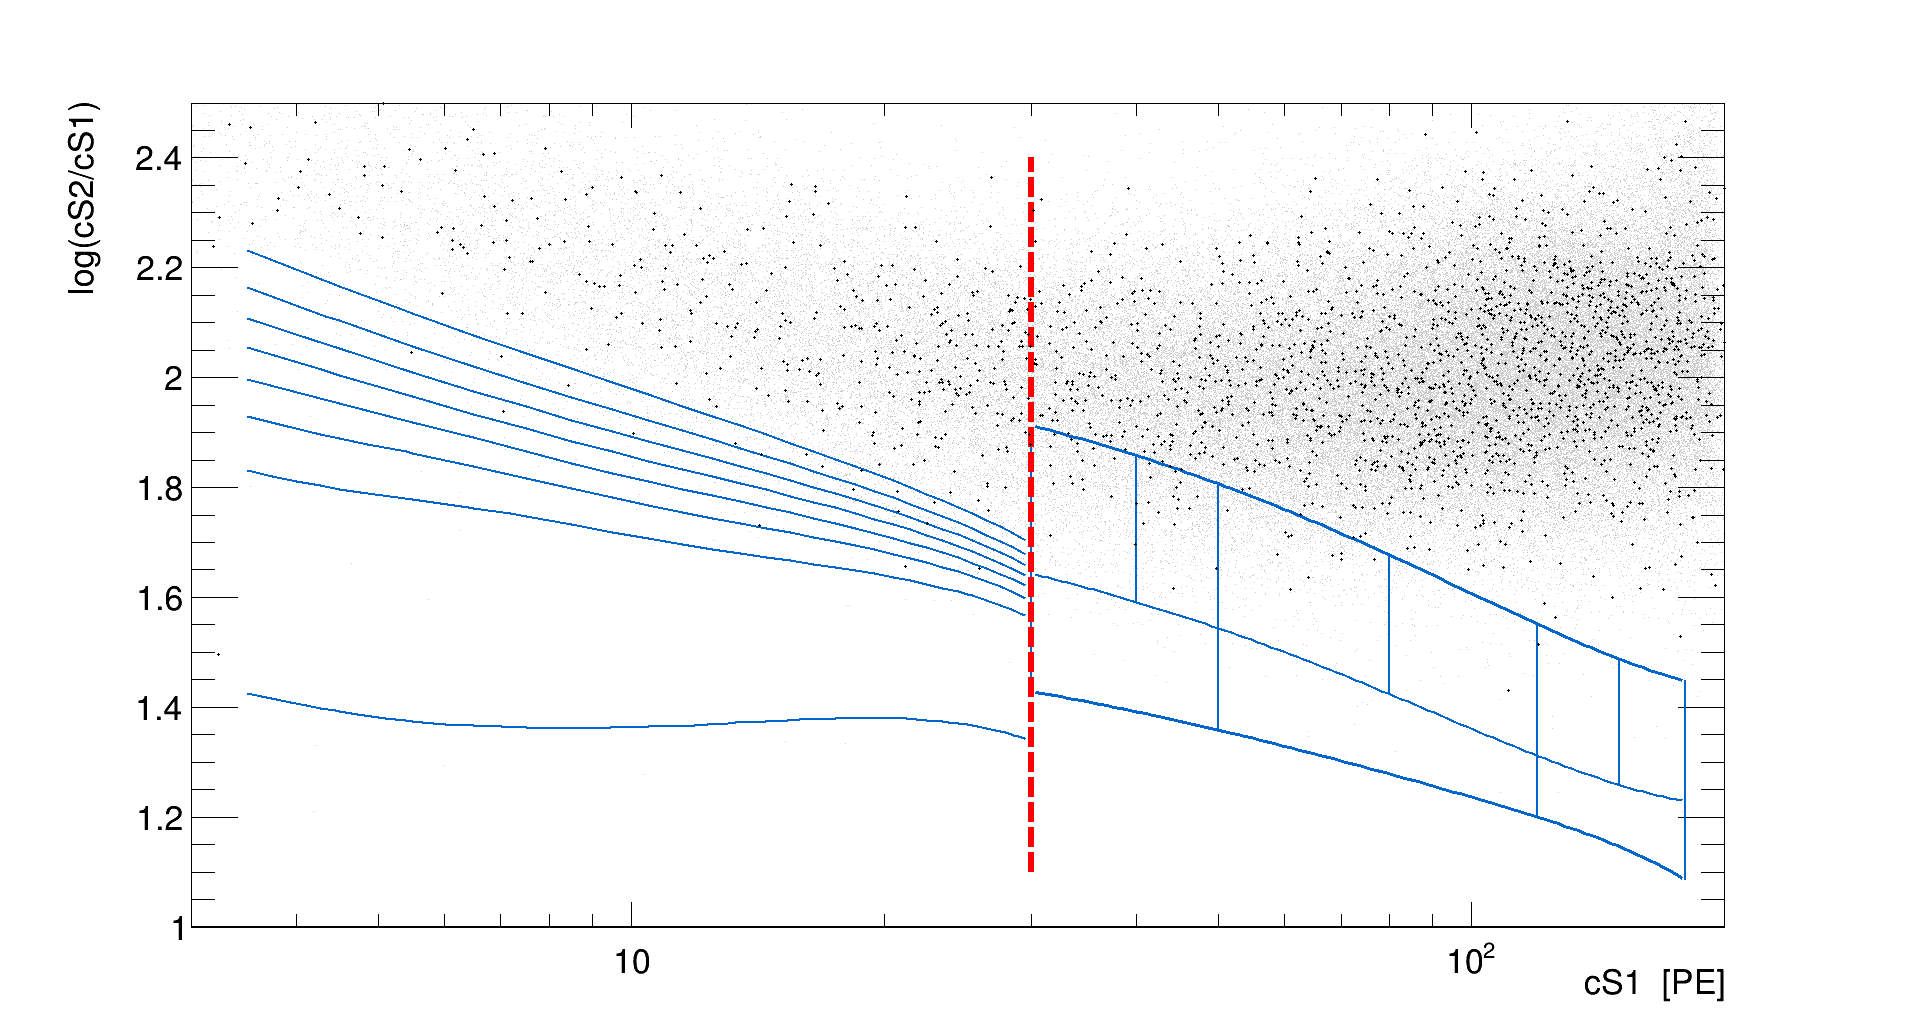
\includegraphics[width=1.\linewidth]{Figures/eft_sr.png}}
\end{minipage}
\caption{$^{Co}$60 and $^{232}$Th data in light gray and DM data in black dots. The upper and lower limits of the energy region are in dotted blue, and the median and bins are in solid.}
\label{fig:phasespace}
\end{figure}  




\subsection{Signal Model}
\label{subsec:SignalModel}
In order to estimate the energy deposition in the high E region we use the \Leff\ based method which is given in Eq.~\ref{eq:LeffEnergyScale}
\begin{equation}
\label{eq:LeffEnergyScale}
	E_{nr} = \frac{cS1}{L_y} \frac{1}{L_{eff}(E_{nr})} \frac{S_{ee}}{S_{nr}}
\end{equation}
The energy range in this region is bounded by the statistics of NR calibration data, namely $^{241}AmBe$.

The signal model is then produced by taking the event rate spectra converting it to S1, applying the acceptance and the detector response (explained in ~\cite{xe100_ana2012}) to give the expected event rate in the detector for each operator see Figure~\ref{fig:HighE}.
\begin{figure}[h!]
\begin{minipage}{1.\linewidth}
\centerline{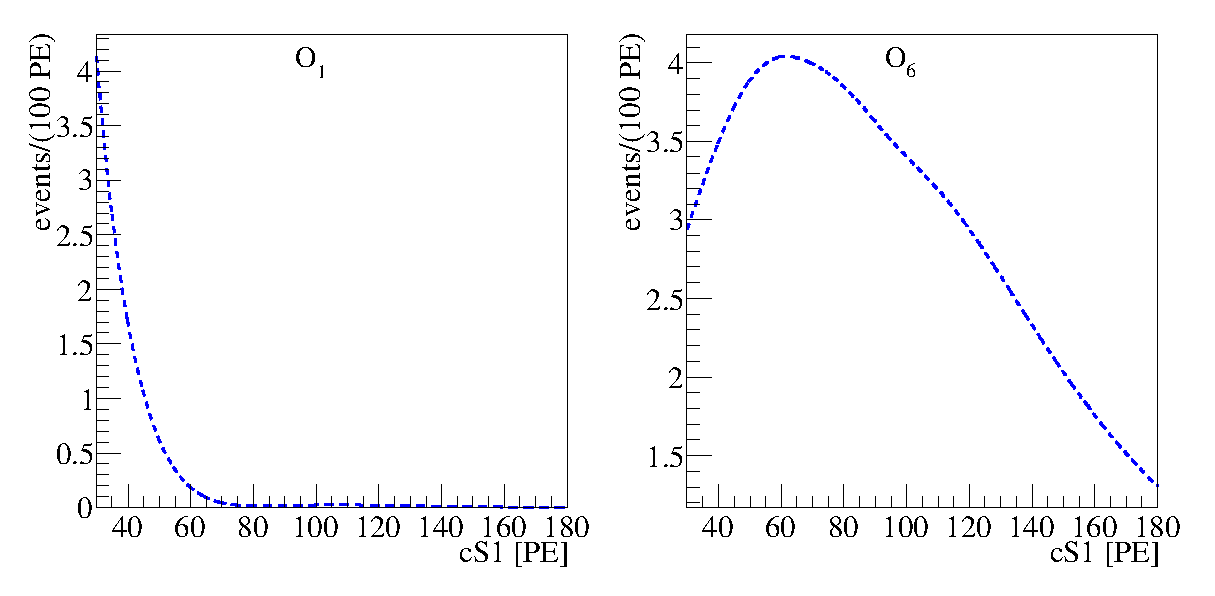
\includegraphics[width=1.\linewidth]{Figures/SigHighO1O6.eps}}
\end{minipage}
\caption{The expected signal in the high energy region for a 300 GeV/$c^2$ WIMP mass, Normalized to 5 events. Left(right) is the spectra for $O_1$($O_6$). Notice that for $O_1$ most of the events are not expected to deposit energy higher then 30 PE whereas for $O_6$ a large fraction of the events appear in this region.}
\label{fig:HighE}
\end{figure} 




\textbf{Ben add here} For the low energy region ...explain shortly the 2D signal model, and give ref to run combination paper. In fig~\ref{fig:LowE} is an example of the expected signal for $O_1$ and $O_6$ normalized to give 5 events in the total energy range (low E and high E)
\begin{figure}[h!]
\begin{minipage}{1.\linewidth}
\centerline{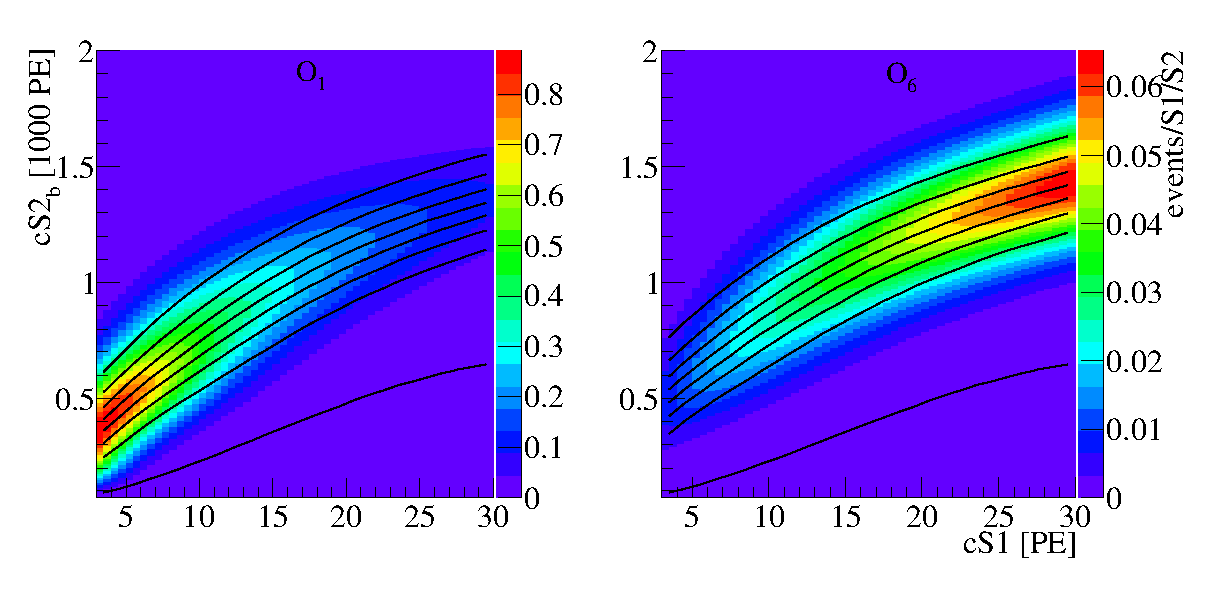
\includegraphics[width=1.\linewidth]{Figures/SigLowO1O6.eps}}
\end{minipage}
\caption{The expected signal in the low energy region for a 300 GeV/$c^2$ WIMP mass, Normalized to 5 events. Left(right) is the spectra for $O_1$($O_6$). Notice that for $O_1$ most of the events are expected to deposit energy lower then 30 PE whereas for $O_6$ a large fraction of the events do not appear in this region at all.}
\label{fig:LowE}
\end{figure}





\subsubsection{Elastic Scattering}
\label{subsubsec:Elastic}
Explain here how to get drde etc. give ref to fitzpatrick
\subsubsection{Inelastic Scattering}
\label{subsubsec:Inelastic}
explain the obtaining of inelastic and give ref to chang


%Explanation of the likelihood methods used, short explaination of the likelihood parts and constraints for combination, joint usage of nuisance parameters {Leff}.

\subsection{The Likelihood Function}
\label{sec:LikelihoodFunction}
The statistical interpretation of data is performed by means of a binned likelihood approach, hypothesis testing rely on a likelihood ratio test statistic, $\tilde{q}$, 
and its asymptotic distributions~\cite{asympt}. The statistical combination between the two analysis channels is achieved merely by the product of the likelihoods,
for the low ($\Llike_{\mathrm{lowE}}$) and high  ($\Llike_{\mathrm{highE}}$) energy channels as shown in equation~\ref{eq:FullLikelihood}. 
Note that the parametrization of the uncertainty related to $\Leff$  is considered correlated between the two channels, as stressed by the common constraint term $\Llike_{\Leff}$.
\begin{equation}
\label{eq:FullLikelihood}
\Llike = \Llike_{\mathrm{lowE}} \times \Llike_{\mathrm{highE}} \times \Llike_{\Leff}
\end{equation}

A binned extended likelihood function is employed for the low energy channel, $\Llike_{\mathrm{lowE}}$, and described in detail in~\cite{xe100_run_combination}, only briefly summarized below.
The ROI for the lowE channel is divided in 8 bands, depending  on the WIMP mass $m_{\chi}$. For each band a term of the type of equation~\ref{} is introduced.

extended Poisson term 

where ns, nb, fs, fb..... tqy and tleff are the parametrization of Leff~\cite{} and Qy~\cite{}. The MLE of the background expectation in each band $\epsilon$ is constrained by the statistical uncertainty 
of the calibration sample in that band.


For the high energy channel a binned likelihood fuction has been chosen, defined in Eq.~\ref{eq:HighELikelihood}
\begin{equation}
\label{eq:HighELikelihood}
\Llike_{\mathrm{highE}}(c_k^2,\Leff) = \prod_{i} \big( Poiss(n^{obs}_{i}~|~n^{s}_{i} + n^{b}_{i}) \, \times Gauss(\eta^{b}_{i}) \big) ~ \times \Llike_{stat}(\epsilon^{s}_{j},\epsilon^{b}_{i}) \times \Llike^s_{unc}(\Leff, A)
\end{equation}
where the product goes over all 9 bins, $\epsilon^{b}_{i}$ is the fraction of background event in \textbf{bin} $i$ and  $\epsilon^{s}_{j}$ is the fraction of AmBe data in \textbf{band} $j$. This means the uncertainty on the signal is assessed per band. $n_i^s = N_{tot}^s(c_k^2,\Leff) \times z_{i,j}^s(\Leff ,\epsilon^{s}_{j})$ is the number of signal events in bin i, $z_{i,j}^s(\Leff, \epsilon^{s}_{j})$ is the fraction of signal events in bin i which is in band j. $n_i^b = N_{tot}^{cal} \times \tau \times \epsilon^{b}_{i}(\eta^{b}_{i})$ is the number of background events in bin i. $\tau$ is the overall normalization of background to data, and is a free parameter.  

The statistical uncertainties on the bins are constrained via:
\begin{equation}
\label{eq:LstsatHighE}
\Llike_{stat}(\epsilon^{s}_{j},\epsilon^{b}_{i}) = \prod_{i}Poiss(N_i^{cal}~|~N_{tot}^{cal} \times \epsilon^{b}_{i}) \times \prod_j Poisson(N_j^{AmBe} | N_{tot}^{AmBe} \times \epsilon^{s}_{j})
\end{equation}
while the uncertainties on the signal model are treated in 
\begin{equation}
\Llike^s_{unc}(\Leff, A) = Gauss(A) \times Gauss(\Leff)
\end{equation}

The uncertainty on the acceptance depend on the expected signal and varies between $\sim$0.01\% to $\sim$7\%. $\eta^{b}_{i}$ is the background systematic uncertainty in bin i and is taken to be 20\%. An additional shape uncertainty due to $\Leff$ is also considered.   

The lowE likelihood function is adopted from previous analyses and is \begin{equation}
\label{eq:LowELikelihood}
\Llike_{lowE} = \Llike_1(c_k^2,\Leff,\Qy) \Llike_2(\epsilon_b) \Llike_3(\Leff,\Qy) .
\end{equation}

\begin{equation} \label{eq:LowELikelihood1}
\begin{split}
\Llike_1(c_k^2,\Leff,\Qy) = &\prod_j Poiss(n^j|\epsilon_s^jM_s(c_k^2)+\epsilon_b^jM_b) \times  \\
&\prod_{i=1}^{n^{i,j}} \frac{\epsilon_s^j M_s(c_k^2)f_s^j(cS1^i) + \epsilon_b^j M_bf_b^j(cS1^i)}{\epsilon^j_sM_s + \epsilon^j_bM_b} ,
\end{split}
\end{equation}

where $f^j_s$ and $f^j_b$ are the probability density functions of the signal and background respectively in band j. and $M_s$ and $M_b$ are the maximum likelihood estimators for the total number of signal and background events respectively.
\begin{equation}
\Llike_2 = \prod_j Poiss(n^j_b | \epsilon_b^jN_b)
\end{equation} 

The last part of the likelihood treats the constraints on the nuisance parameter $\Qy$ and $\Leff$ normally constraining them. The latter is a joined nuisance parameter for both energy regions. 


Explanation of the likelihood methods used, short explaination of the likelihood parts and constraints for combination, joint usage of nuisance parameters {Leff}.
%\subsubsection{High Energy}
%likelihood function + uncertainties 
%\subsubsection{Low Energy}
%ref to run combination.






\section{Results}
\subsection{Elastic Scattering}
\RanComment{ A benchmark region of interest is defined similarly to~\cite{xe100_run_combination}, between the upper and lower
thresholds in cS1 for each channel. This region
is bounded in y space from above by the 99.75\% ER rejection line and below by the lower 3$\sigma$ quantile of the AmBe neutron calibration data. The expected background in the region is $1.7 \pm 0.3$ (lowE) and $1.49 \pm 0.25$ (highE). The number of DM candidates recorded in this region is 1 (lowE), and 0 (highE). }
sout{A total of 50 events are recorded in the signal region distributed in the bins as defined in Table~\ref{table:BinDef}.} The data is compatible with background only hypothesis and no excess is found. For all operators and masses in the range of 10 Gev/$c^2$ to 1TeV$c^2$, \Xehund\ sets the strongest limits on the effective coupling constant $c_i$. These limits are shown in Fig.~\ref{fig:elasticLimit} in black, along with the limits from CDMS-II Si, CDMS-II Ge and SuperCDMS~\cite{CDMSEFT}. For operators 3 and 8, a full CDMS limit is presented, for all other operators only the limit for a 10 GeV/$c^2$ and 300 GeV/$c^2$ are published.  

\begin{figure*}
\begin{minipage}{1.\linewidth}{}
\centerline{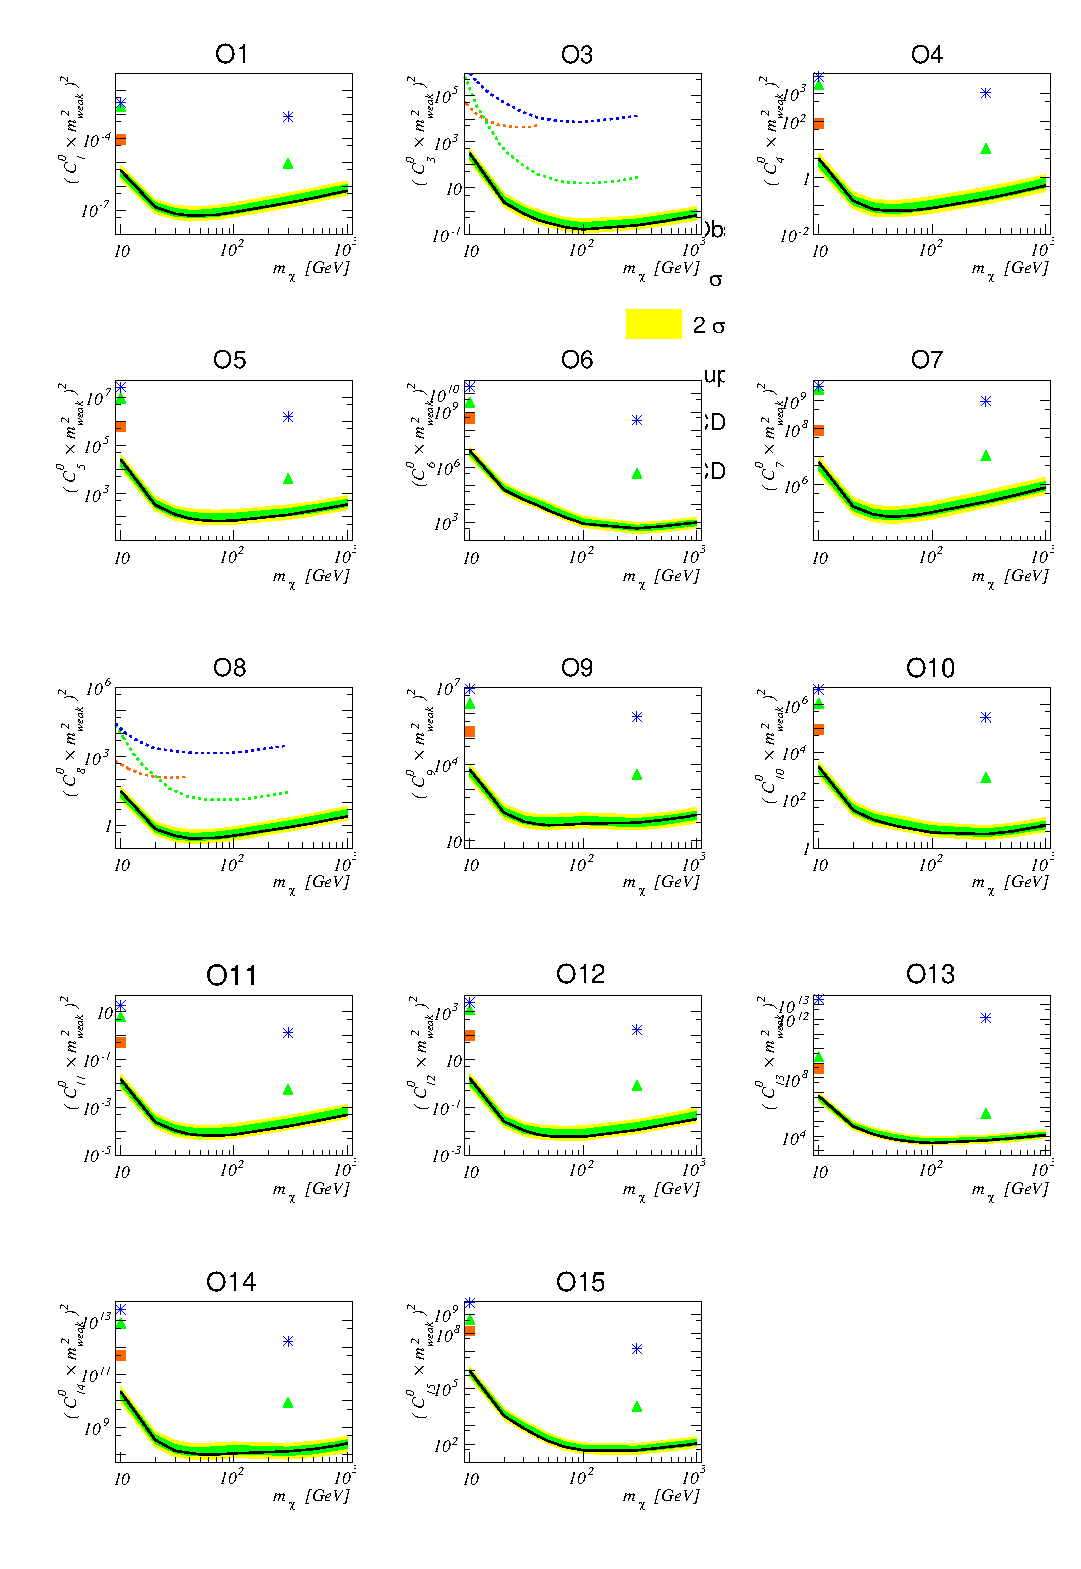
\includegraphics[width=\textwidth,height=\textheight,keepaspectratio]{Figures/SizeTestCDMS.eps}}
%{Figures/ElasticAllLimitCDMS.eps}}
\end{minipage}
\caption{The \Xehund\ limits (90\% CL) Limits on isoscalar dimensionless coupling for all elastic scattering EFT operators are indicated in solid black. The expected sensitivity obtained assuming background only are is shown in green and yellow(1$\sigma$ and 2$\sigma$ respectively). Limits from CDMS-II Si CDMS-II Ge and SuperCDMS cite{CDMS} are presented in blue Astrix ,green triangle and orange rectangle (color online). For operator 3 and 8 a full limit from CDMS is published and indicated by a dashed line in the respected colors.}
\label{fig:elasticLimit}
\end{figure*}


\subsection{Inelastic Scattering}
The limit of inelastic scattering for the SI case ($\mathcal{O}_1$) is shown both as a function of mass splitting and WIMP mass in Fig.~\ref{fig:O1Inel}. Each line represents the 90\% CL for a specific coupling constant value. 

The limits for all other operators are calculated for a WIMP mass of 1 TeV/$c^2$ as a function of the mass splitting $\delta_m$ (Fig.~\ref{fig:InelasticLimit}) 
\begin{figure}[h!]
\centerline{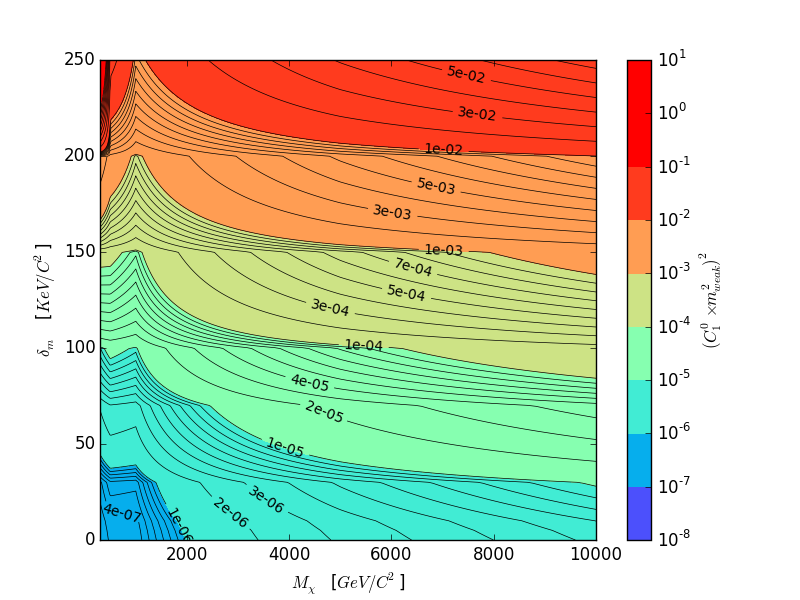
\includegraphics[width=1.\linewidth]{Figures/inelastic_delta_vs_m.png}}
\caption{90\% confidence level limits on coupling constant for $\mathcal{O}_1$ reported as a function of the WIMP mass and mass splitting $\delta$.}
\label{fig:O1Inel}
\end{figure}  



\begin{figure*}
\begin{minipage}{1.\linewidth}
\centerline{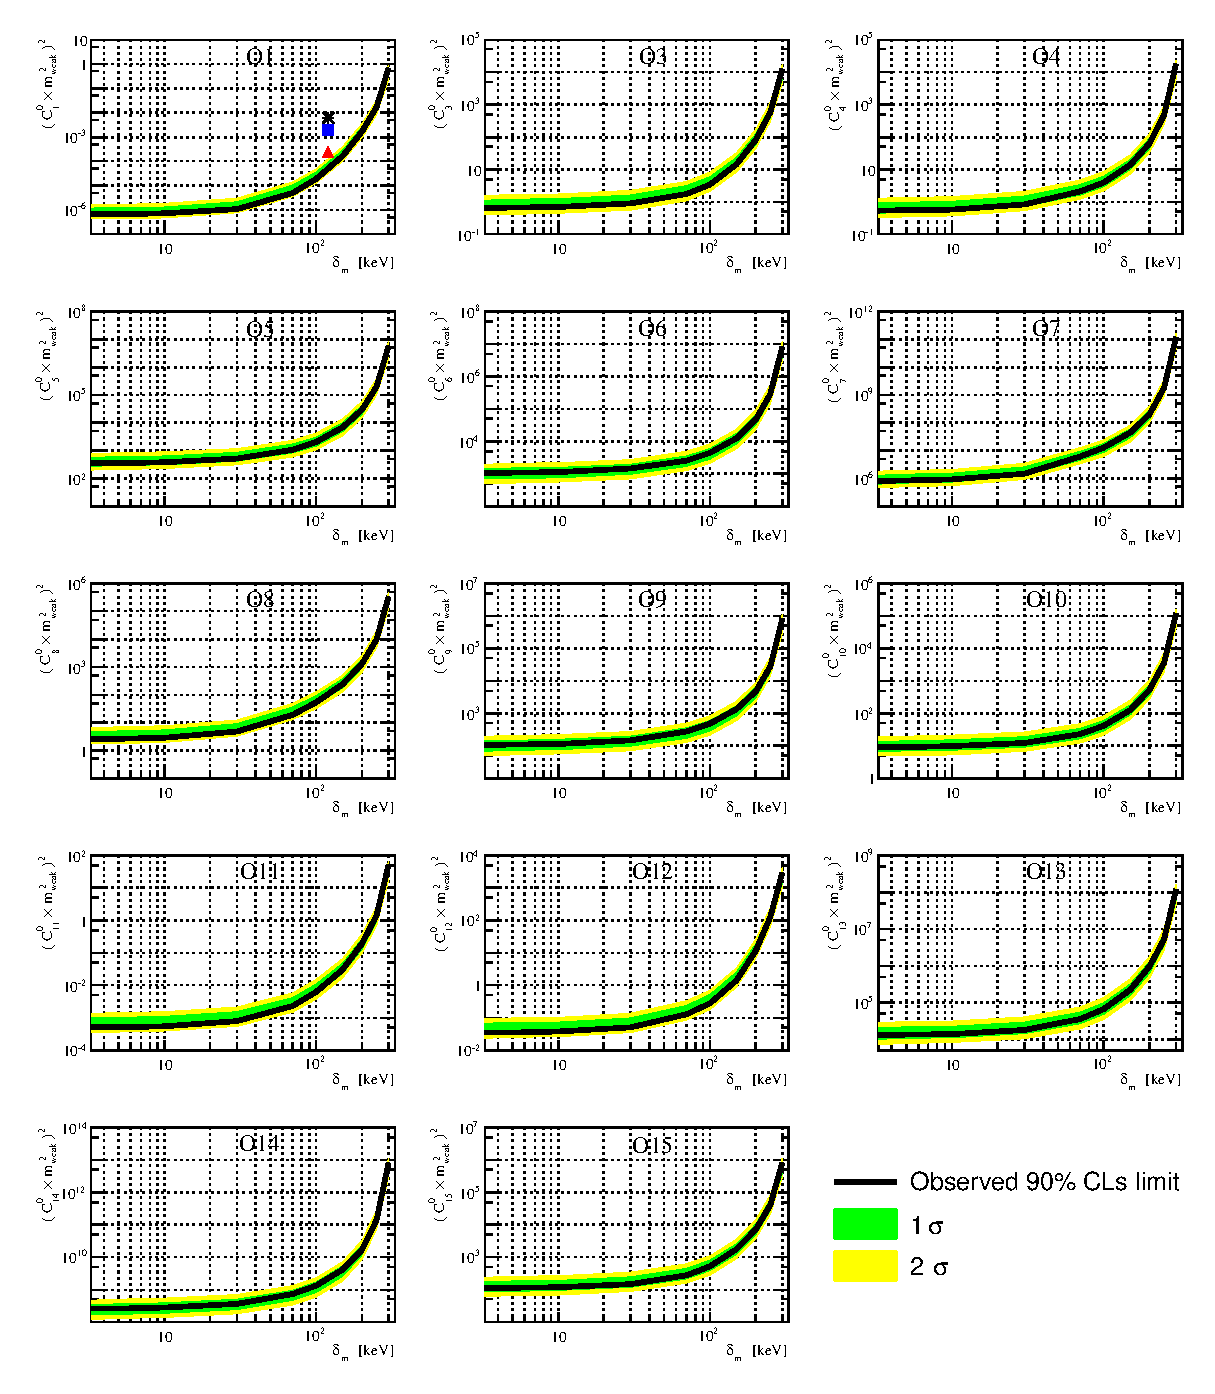
\includegraphics[width=\textwidth,height=\textheight,keepaspectratio]{Figures/FinalInelastic.eps}}
\end{minipage}
\caption{The \Xehund\ limits (90\% CL) Limits on a 1 TeV/$c^2$ WIMP isoscalar dimensionless coupling for all inelastic scattering EFT operators are indicated in solid black. The expected sensitivity obtained assuming background only are is shown in green and yellow(1$\sigma$ and 2$\sigma$ respectively). }
\label{fig:InelasticLimit}
\end{figure*}

\FloatBarrier


\section{Summary}
We have shown the first analysis of \Xehund\ data at recoil energies above 43 keV, with the new high energy bound set to 240 keV. We considered in this paper two models which predict interactions in this energy region: an EFT approach for elastic WIMP-nucleon scattering, and a similar EFT approach but considering instead inelastic WIMP-nucleon scattering. The observed data was compatible with background expectations, and 90\%\,CL$_S$ exclusion limits were constructed for WIMP masses between 10-1000 GeV.

\section{Acknowledgment}
Liam Fitzpatrick
Spencer Chang

%\newpage



\appendix*

\section{Signal model detector response table}

In this appendix we describe digital tables which can be used to construct an accurate signal model for this analysis given any input recoil spectrum $\mathrm{d}R/\mathrm{d}E$ arising from a theoretical model. A visualization of the tables is shown in Fig.~\ref{fig:smeartable_highE}, and in section \ref{app:example_code} we show a simple example Python code of how to use the supplied tables. Currently we provide these tables only for the high-energy analysis region.

The signal model for the high-energy analysis region can be expressed analytically in the form:
%
\begin{align}
\label{eq:high2D}
  \frac{\mathrm{d} R}{\mathrm{d}\cSi} &= \int \! \frac{\mathrm{d}R}{\mathrm{d}E} \cdot \epsilon_\mathrm{S1}(\cSi) \cdot \epsilon_\mathrm{S2'}(E) \cdot p_\mathrm{S1}(\mathrm{\cSi}|E) \, \mathrm{d}E \\
  &= \int \! \frac{\mathrm{d}R}{\mathrm{d}E} G(\cSi,E) \, \mathrm{d}E
\end{align}
%
where $\epsilon_\mathrm{S1}(\cSi)$ and $\epsilon_\mathrm{S2'}(E)$ represent analysis cut efficiencies, $p_\mathrm{S1}(\mathrm{\cSi}|E)$ encodes detector effects, and $\mathrm{d}R/\mathrm{d}E$ gives the theoretically predicted nuclear recoil rate from WIMP scattering. In the second line we emphasis that all the detector and analysis effects can be encoded in a single function $G(\cSi,E)$. To make a signal prediction for the bins in our analysis, this expression needs to be integrated over the appropriate range of $\cSi$ for each bin (and divided by two to account for the banding structure in $\cSiib$):
%
\begin{equation}
  R_\mathrm{bin_i} = \frac{1}{2}\int_{\mathrm{lower}_i}^{\mathrm{upper}_i} \! \frac{\mathrm{d} R}{\mathrm{d}\cSi} \, \mathrm{d}\cSi
\end{equation}
%
With some simple rearrangement this rate can be written in terms of an integral over the detector response function $G$ as follows
%
\begin{align}
  R_\mathrm{bin_i} &= \frac{1}{2}\int\frac{\mathrm{d} R}{\mathrm{d}E}\int_{\mathrm{lower}_i}^{\mathrm{upper}_i} \! G(\cSi,E) \, \mathrm{d}\cSi \, \mathrm{d}E \\
 &= \int\frac{\mathrm{d} R}{\mathrm{d}E} G'_i(E) \mathrm{d}E
\end{align}
%
where in the last line we absorb the factor of $1/2$ into the definition of $G'_i$. We see here that the signal rate for each bin can be expressed as an integral over the recoil spectrum times a detector response function $G'_i$ for that bin. It is these detector response functions which are shown in Fig.~\ref{fig:smeartable_highE}, and which we provide digitally for use by the community. A low-resolution example is given in Table \ref{tab:smeartable_highE}. With these tables it is simple to produce a signal model for our analysis for any theoretical recoil spectrum. The functions $G'_i$ are provided for three values of the nuisance variable $\Leff$, namely the median value and values at $\pm 1 \sigma$ in $\Leff$. From these, along with the measured background rates given in table \ref{table:BinDef}, one may construct a likelihood which accounts for uncertainties in $\Leff$, Alternatively simply using the $-1\sigma$ value produces quite an accurate prediction and is generally conservative.

\begin{figure}
\centerline{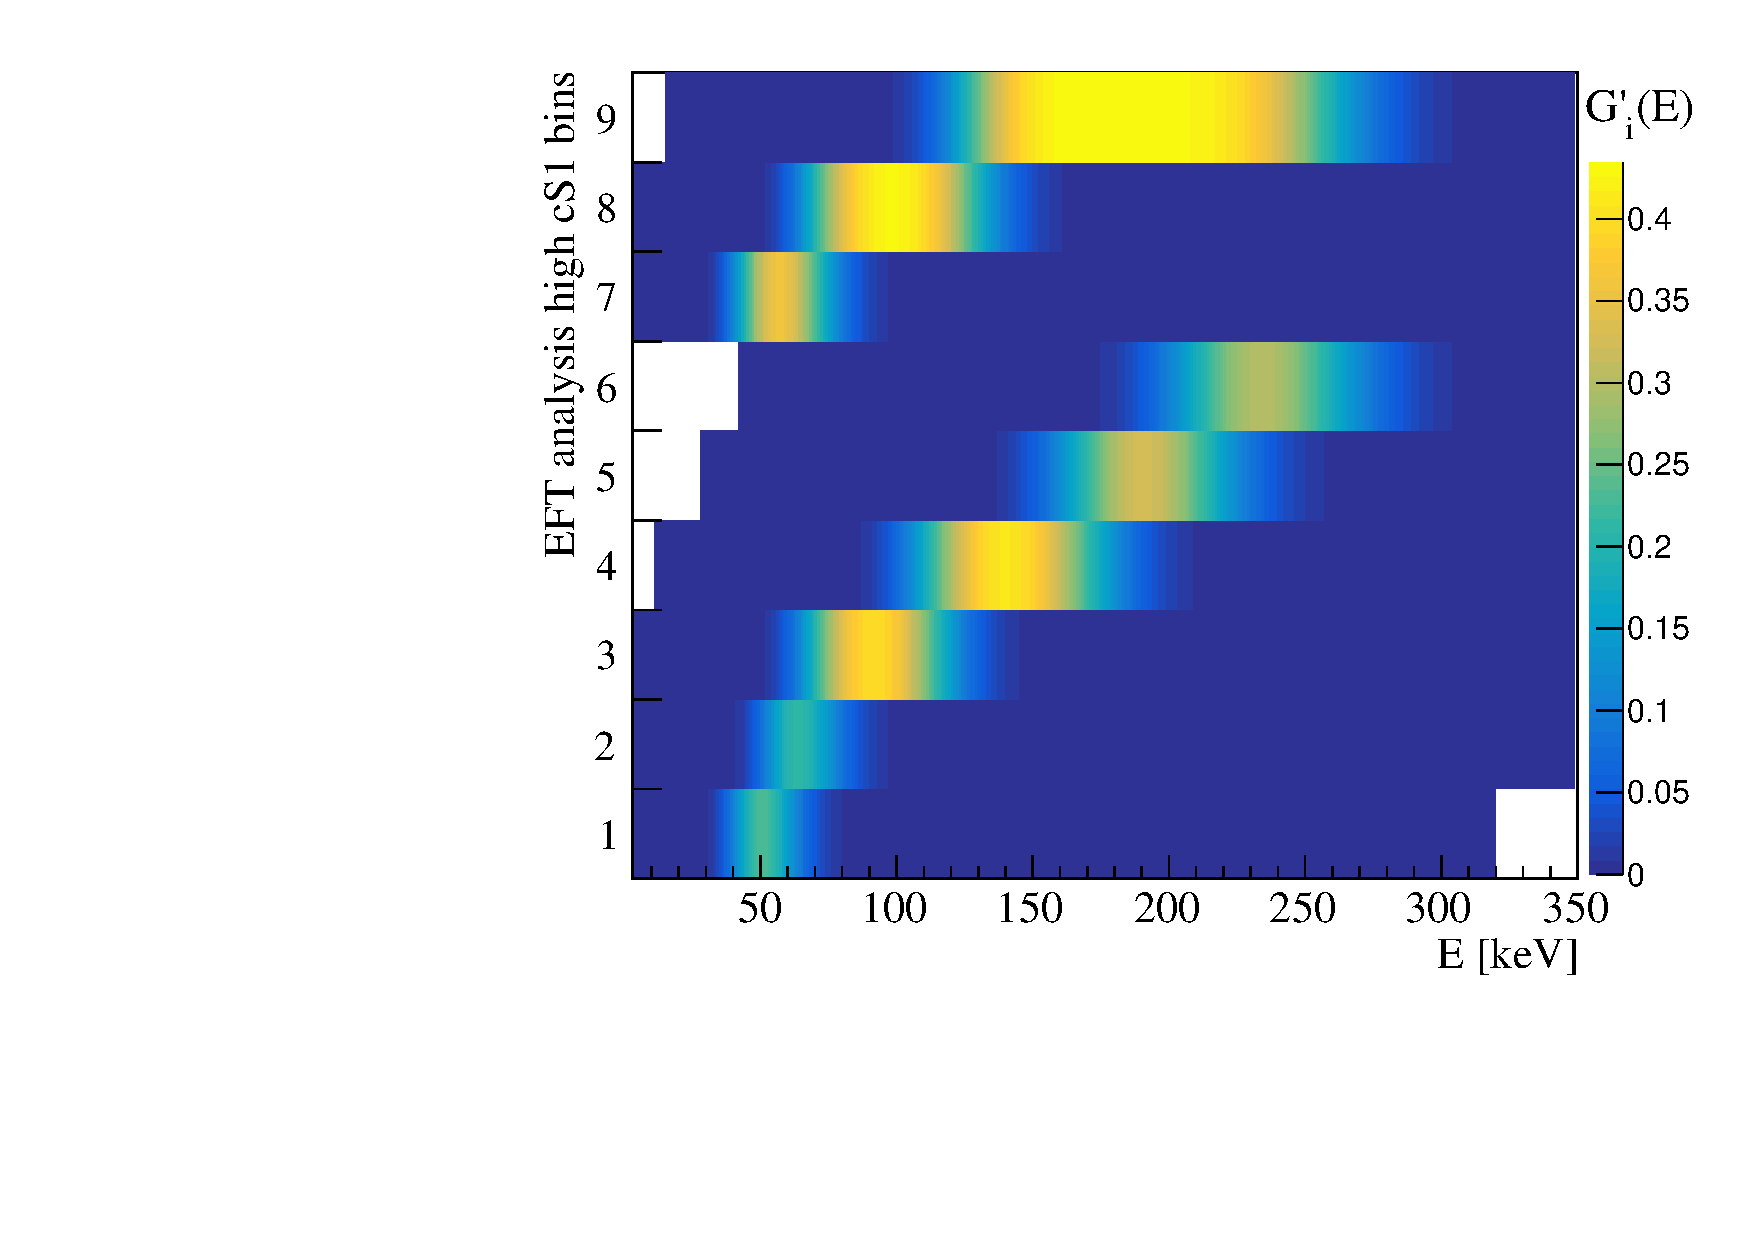
\includegraphics[width=1.\linewidth]{Figures/smeartable_highE}}
\caption{A visualization of the detector response table for $-1\sigma$ (i.e. conservative) $\Leff$, as provided in the supplementary material. The y axis indicates the bins used for the high-energy signal region of this analysis (explained in ~\ref{table:BinDef}). The $x$ axis shows recoil energies, and the colors give the probability density for a recoil of a given recoil energy to produce an event in each analysis bin. To produce a signal model for this analysis, one simply multiplies the table values by $\mathrm{d}R/\mathrm{d}E$ and integrates over $E$. The result is the predicted signal rate for each analysis bin.}
\label{fig:smeartable_highE}
\end{figure}  

\begin{table}
{
  \lstset{tabsize=4,basicstyle=\tiny\ttfamily,columns=flexible,emptylines=10000,keepspaces=true}
  \lstinputlisting{smeartable_Leff-1.dat}
}
\caption{Detector response table using $\Leff$ with constrained scaling parameter set to $-1\sigma$ value. First column gives recoil energies, subsequent columns give the values of $G'_i(E)$ for each of the 9 high-energy analysis bins. The sampling is in steps of $10~\keVr$, which is too coarse to give an accurate signal model for very low WIMP masses, but is suitable for the mass range most relevant to our analysis. Higher resolution $G'_i(E)$ functions, and $G'_i(E)$ functions for other values of $\Leff$, are given in supplementary material \BenComment{give URL}. 
\label{tab:smeartable_highE}
}
\end{table}  
%\newpage
\subsection{Example code}
\label{app:example_code}
\begin{lstlisting}
import numpy as np
from numpy import newaxis
from scipy.interpolate import interp1d

def TrapI(x,y):
    """Simple trapezoid integration"""
    w = x[1:] - x[:-1]
    h = (y[1:] + y[:-1])/2.
    return np.sum(w*h,axis=0)

# Load detector response table
data = np.loadtxt("detector_table.dat")
E = data[:,0]; Gi = data[:,1:]

# Load test recoil spectrum (1 TeV WIMP, O6)
data = np.loadtxt("O6_1TeV.dat")
Er = data[:,0]
# Input spectra is normalised to coupling^2=1,
# rescale to something near limit (1e3)
# Also multiply in the appropriate exposure
dRdE = data[:,1] * (1e3/1.) * 224.6*34.
# Interpolate recoil spectrum to table values
# Assume spectrum zero outside data given
f_dRdE = interp1d(Er,dRdE)
dRdE_matched = f_dRdE(E)
Ri = TrapI(E[:,newaxis],Gi*dRdE_matched[:,newaxis])

for i,R in enumerate(Ri):
  print "bin {0}: rate = {1:.2g}".format(i+1,R)

Output:

bin 1: rate = 0.081
bin 2: rate = 0.098
bin 3: rate = 0.35
bin 4: rate = 0.46
bin 5: rate = 0.29
bin 6: rate = 0.22
bin 7: rate = 0.18
bin 8: rate = 0.47
bin 9: rate = 0.84
\end{lstlisting}

%\vfill







%%% BIBLIOGRAPHY %%%


\bibliography{EFTPaperBib}

\end{document}
